
\chapter{Measurement of Planck's Constant}

\section{Introduction}

In this lab, we will measure Planck's constant by measure the $V$-$I$ curves of three different colored light emitting diodes.

\section{$V-I$ Curve from LED.}

\begin{figure}[htbp]
\begin{center}
\begin{circuitikz}[line width=1pt]
\draw (0,0) to[voltage source,bipoles/length=1.5cm,l=$V_1$] ++(0,4.0) to[short] ++(2.0,0) coordinate(C);
\draw (C) to[R, l_=$R_1$] ++(0,-2.0) coordinate(B) to[empty diode, l_=LED] ++(0,-2.0) coordinate(A) to[short] ++(-2.0,0.0);
\draw (A) to[short,*-] ++(1.5,0) to[short] ++(0,0.8) node[component]{V} to[short] ++(0,0.8) to[short,-*] ++(-1.5,0);
\draw (C) to[short,*-] ++(1.5,0) to[short] ++(0,-0.8) node[component]{V} to[short] ++(0,-0.8) to[short,-*] ++(-1.5,0);
\end{circuitikz} 
\end{center}
\caption{experimental setup.}
\label{fig:planck_setup}
\end{figure}

Construct the experimental setup shown in Fig.~\ref{fig:planck_setup}
using a $1~\rm k\Omega$ precision $1\%$ resistor for $R_1$, a green
LED, and using your bench-top DC supply to provide $V_1$, initially
set to $0~\rm V$.  Connect one voltmeter across the resistor $R_1$ and
another voltmeter across the LED.  When constructing your circuit,
make sure the LED can be easily removed and replaced.  Also keep in
mind that the longer lead is the positive terminal of the LED, i.e.,
the upper terminal of the LED as drawn in the
Fig.~\ref{fig:planck_setup}.  Set both voltmeters to the $20~\rm V$
setting.


Test your circuit first by turning up the voltage on your supply to
about $5~\rm V$ and checking that the LED lights up.  The voltmeter
across the resistor $R_1=1~\rm k\Omega$ is effectively measuring the
current in $mA$ as $1~{\rm V}/1~{\rm k\Omega} = 1~\rm mA$.  Do not
misunderstand this statement to mean you should set the multi-meter to
the current measurement: we measure the voltage, but from $Ohm's Law$
we know the current in resistor.  The voltmeter across the diode is
measuring the diode drop $V_{\rm D}$.

Take a series of measurements of $I$ and $V_D$ near target values of
$I = 0.5,1.0,2.0,4.0,6.0,8.0,10.0,12.0~\rm mA$ by adjusting the
voltage provided by your DC supply until the current $I$, as measured
with the voltmeter across $R_1$, is near the target value.  Remember
not to waste time fussing to make the measurement at exactly the
target value.  For instance, measuring at $I=2.16~\rm mA$ instead of
the target $I=2.0 ~\rm mA$ is perfectly acceptable.  Simply record the
actual measured value of $I$ next to target value, in addition to
measurement of $V_{\rm D}$.  

\begin{table}
\begin{center}
\caption{Example data from an LED not used in this experiment.}
\begin{tabular}{lll}
target $I$ (mA) & $I$ (mA) & $V_{\rm D}$ (V) \\
\hline
0.5 &  0.51 & 2.83 \\
1   &  1.00 & 3.08 \\
2   &  2.00 & 3.35 \\
4   &  4.08 & 3.68 \\
6   &  6.07 & 3.87 \\
8   &  8.00 & 4.01 \\
10  & 10.03 & 4.12 \\
12  & 12.03 & 4.21 \\
\end{tabular}
\end{center}
\end{table}

Repeat this measurement using a green and yellow LED.

\begin{table}[htbp]
\begin{center}
\caption{LEDs used in this experiment.}
\begin{tabular}{llll}
color & part no. & $\lambda$ (nm) & max current \\
%blue  & WP710A10QBC & 460 & 30 mA \\
green & WP710A10GT & 565 & 25 mA \\  
yellow & TLHY4405 & 581-594 & 30 mA \\ 
red & TLHR4405 & 612-625 & 30 mA \\ 
\end{tabular}
\end{center}
\end{table}

\section{Analysis}

\begin{figure}[htbp]
\begin{center}
%\begin{tabular}{cc}
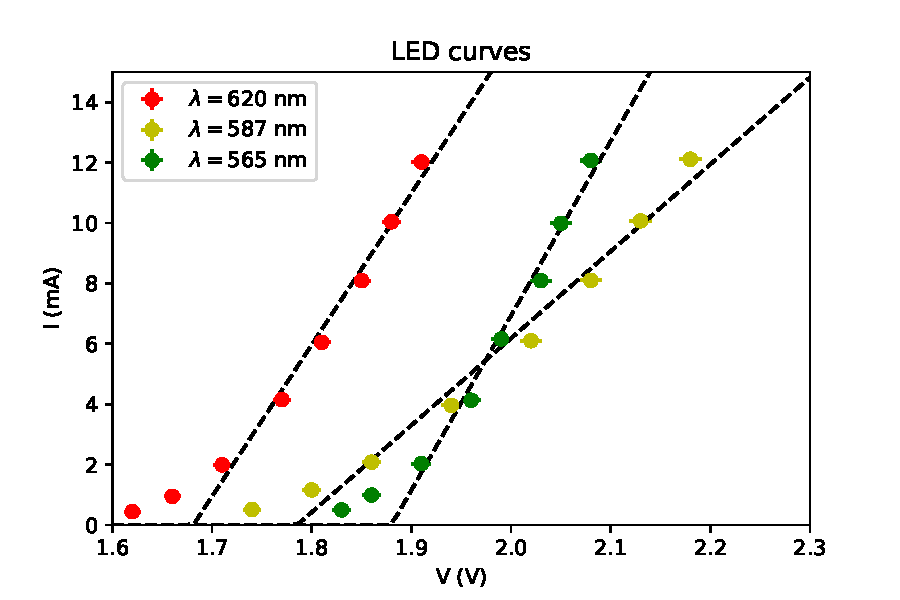
\includegraphics[height=0.3\textheight]{figs/labs/planck/led_curves.pdf} \\
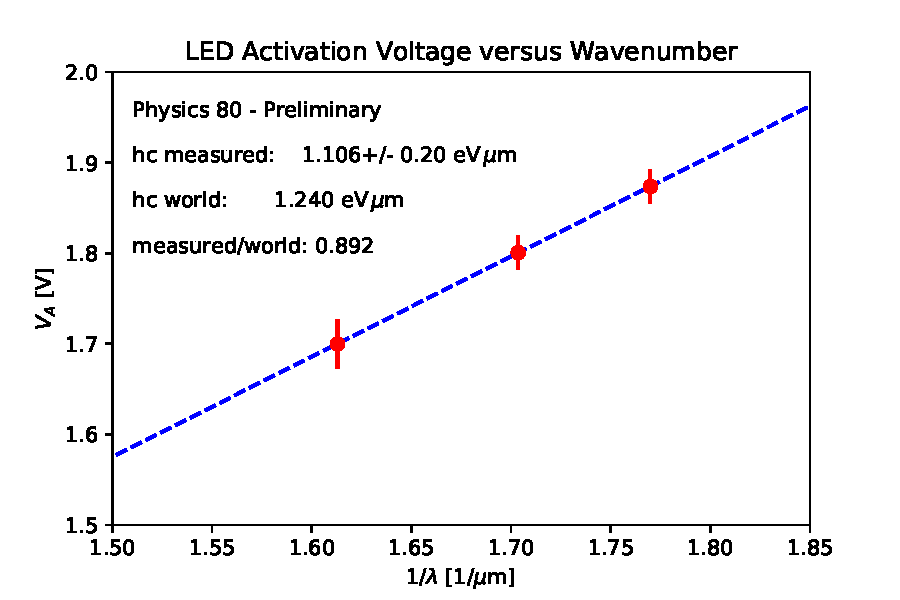
\includegraphics[height=0.3\textheight]{figs/labs/planck/planck.pdf} \\
%\end{tabular}
\end{center}
\caption{Instructor plots from Data Analysis.}
\label{fig:planck_setup}
\end{figure}
